\section[Releases/Program Increment]{Releases/Program Increment}
A equipe optou por definir Releases e Program Increment como sendo a mesma coisa dentro do projeto. Foram planejadas duas releases, com as datas de entrega no dia 17/11/2016 da Primeira Release e dia 17/12/2016 para Segunda Release. 

Como a release é um item de planejamento em nível de programa, ele tem como base alocações de features. 

A equipe de desenvolvimento tentou distribuir os pontos de forma semelhante nas duas releases, porém, de acordo com a priorização das funcionalidades por parte da cliente, a Primeira Release teve uma pontuação maior, como pode ser observada nas imagens abaixo.

\begin{figure}[!htb]
    \centering
    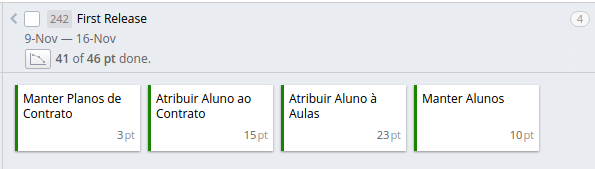
\includegraphics[width=\textwidth]{figuras/release_1.png}
    \caption{Quadro Primeira Release}
    \label{fig:release_1}
\end{figure}

\begin{figure}[!htb]
    \centering
    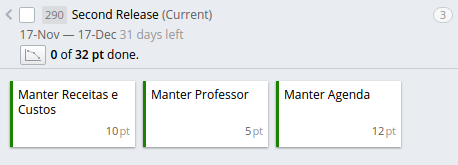
\includegraphics[width=\textwidth]{figuras/release_2.png}
    \caption{Quadro Segunda Release}
    \label{fig:release_2}
\end{figure}